\documentclass[14pt,a4paper,report]{report}
\usepackage[a4paper, mag=1000, left=2.5cm, right=1cm, top=2cm, bottom=2cm, headsep=0.7cm, footskip=1cm]{geometry}
\usepackage[utf8]{inputenc}
\usepackage[english,russian]{babel}
\usepackage{indentfirst}
\usepackage[dvipsnames]{xcolor}
\usepackage[colorlinks]{hyperref}
\usepackage{listings} 
\usepackage{fancyhdr}
\usepackage{caption}
\usepackage{amsmath}
\usepackage{latexsym}
\usepackage{graphicx}
\usepackage{amsmath}
\usepackage{booktabs}
\usepackage{array}
\hypersetup{
	colorlinks = true,
	linkcolor  = black
}

\usepackage{titlesec}
\titleformat{\chapter}
{\Large\bfseries} % format
{}                % label
{0pt}             % sep
{\huge}           % before-code


\DeclareCaptionFont{white}{\color{white}} 

% Listing description
\usepackage{listings} 
\DeclareCaptionFormat{listing}{\colorbox{gray}{\parbox{\textwidth}{#1#2#3}}}
\captionsetup[lstlisting]{format=listing,labelfont=white,textfont=white}
\lstset{ 
	% Listing settings
	inputencoding = utf8,			
	extendedchars = \true, 
	keepspaces = true, 			  	 % Поддержка кириллицы и пробелов в комментариях
	language = C++,            	 	 % Язык программирования (для подсветки)
	basicstyle = \small\sffamily, 	 % Размер и начертание шрифта для подсветки кода
	numbers = left,               	 % Где поставить нумерацию строк (слева\справа)
	numberstyle = \tiny,          	 % Размер шрифта для номеров строк
	stepnumber = 1,               	 % Размер шага между двумя номерами строк
	numbersep = 5pt,              	 % Как далеко отстоят номера строк от подсвечиваемого кода
	backgroundcolor = \color{white}, % Цвет фона подсветки - используем \usepackage{color}
	showspaces = false,           	 % Показывать или нет пробелы специальными отступами
	showstringspaces = false,    	 % Показывать или нет пробелы в строках
	showtabs = false,           	 % Показывать или нет табуляцию в строках
	frame = single,              	 % Рисовать рамку вокруг кода
	tabsize = 2,                  	 % Размер табуляции по умолчанию равен 2 пробелам
	captionpos = t,             	 % Позиция заголовка вверху [t] или внизу [b] 
	breaklines = true,           	 % Автоматически переносить строки (да\нет)
	breakatwhitespace = false,   	 % Переносить строки только если есть пробел
	escapeinside = {\%*}{*)}      	 % Если нужно добавить комментарии в коде
}

\begin{document}

\def\contentsname{Содержание}

% Titlepage
\begin{titlepage}
	\begin{center}
		\textsc{Санкт-Петербургский Политехнический 
			Университет Петра Великого\\[5mm]
			Кафедра компьютерных систем и программных технологий}
		
		\vfill
		
		\textbf{Отчёт по лабораторной работе №5\\[3mm]
			Курс: «Администрирование компьютерных сетей»\\[3mm]
			Тема: «Создание макета сети в Cisco Packet Tracer»\\[35mm]
			}
	\end{center}
	
	\hfill
	\begin{minipage}{.5\textwidth}
		Выполнил студент:\\[2mm] 
		Бояркин Никита Сергеевич\\
		Группа: 13541/3\\[5mm]
		
		Проверил:\\[2mm] 
		Малышев Игорь Алексеевич
	\end{minipage}
	\vfill
	\begin{center}
		Санкт-Петербург\\ \the\year\ г.
	\end{center}
\end{titlepage}

% Contents
\tableofcontents
\clearpage

\chapter{Лабораторная работа №5}

\section{Цель работы}

\begin{itemize}
	\item Ознакомиться с Cisco Packet Tracer.
	\item Построить в Packet Tracer компьютерную сеть.
	\item Настроить сервисы DNS, DHCP, TFTP.
	\item Протестировать сеть.
\end{itemize}

\section{Создание макета сети в Cisco Packet Tracer}

Необходимо построить следующую компьютерную сеть:

\begin{figure}[h!]
	\centering
	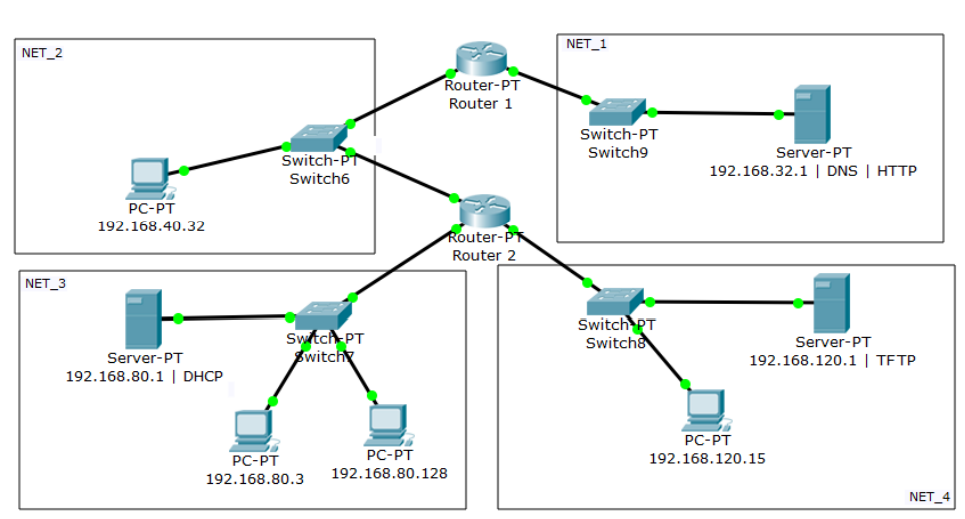
\includegraphics[scale = 0.65]{images/0.png}
	\caption{Проектируемая компьютерная сеть}
	\label{image:0}
\end{figure}

\clearpage

\subsection{Настройка сети}

\subsubsection{Настройка подсети NET\_1}

\begin{figure}[h!]
	\centering
	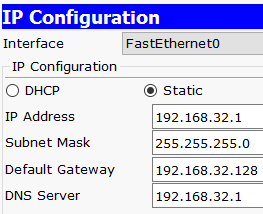
\includegraphics[scale = 0.85]{images/1.png}
\end{figure}

\subsubsection{Настройка роутера 1}

\begin{figure}[h!]
	\centering
	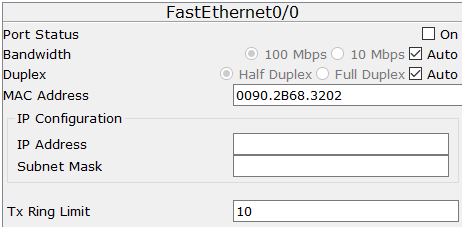
\includegraphics[scale = 0.85]{images/2_1.png}
\end{figure}

\begin{figure}[h!]
	\centering
	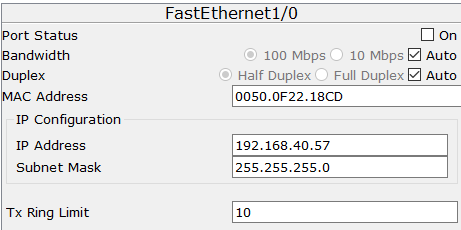
\includegraphics[scale = 0.85]{images/2_2.png}
\end{figure}

\begin{figure}[h!]
	\centering
	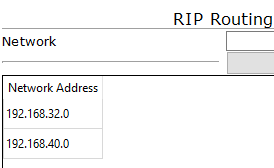
\includegraphics[scale = 0.85]{images/2_3.png}
\end{figure}

\clearpage

\subsubsection{Настройка подсети NET\_2}

\begin{figure}[h!]
	\centering
	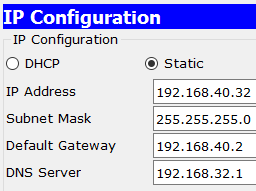
\includegraphics[scale = 0.85]{images/3.png}
\end{figure}

\subsubsection{Настройка роутера 2}

\begin{figure}[h!]
	\centering
	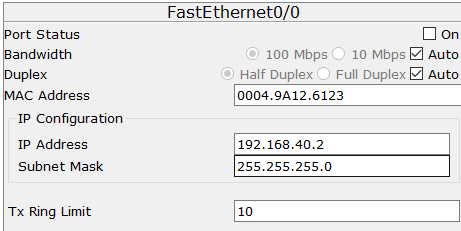
\includegraphics[scale = 0.85]{images/4_1.png}
\end{figure}

\begin{figure}[h!]
	\centering
	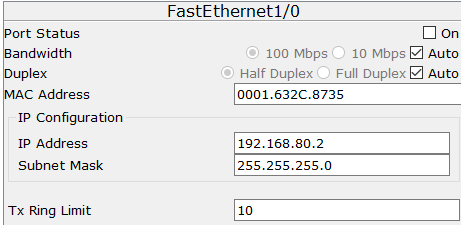
\includegraphics[scale = 0.85]{images/4_2.png}
\end{figure}

\begin{figure}[h!]
	\centering
	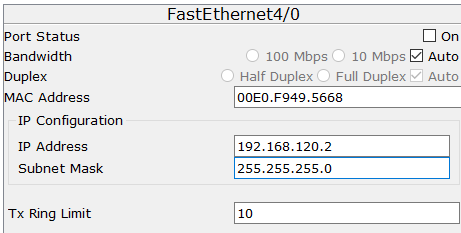
\includegraphics[scale = 0.85]{images/4_3.png}
\end{figure}

\clearpage

\begin{figure}[h!]
	\centering
	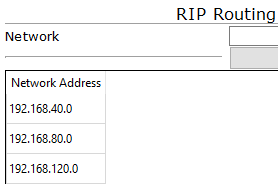
\includegraphics[scale = 0.85]{images/4_4.png}
\end{figure}

\subsubsection{Настройка подсети NET\_3}

\begin{figure}[h!]
	\centering
	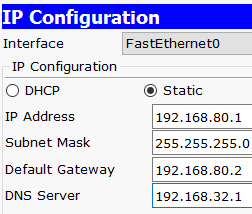
\includegraphics[scale = 0.85]{images/5_1.png}
\end{figure}

\begin{figure}[h!]
	\centering
	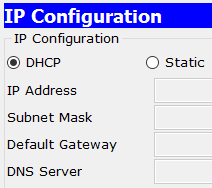
\includegraphics[scale = 0.85]{images/5_2.png}
\end{figure}

\begin{figure}[h!]
	\centering
	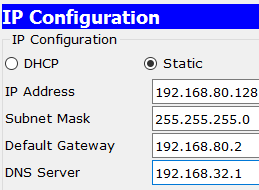
\includegraphics[scale = 0.85]{images/5_3.png}
\end{figure}

\clearpage

\subsubsection{Настройка подсети NET\_4}

\begin{figure}[h!]
	\centering
	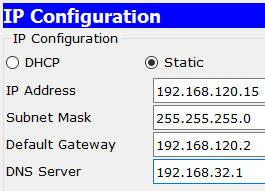
\includegraphics[scale = 0.85]{images/6_1.png}
\end{figure}

\begin{figure}[h!]
	\centering
	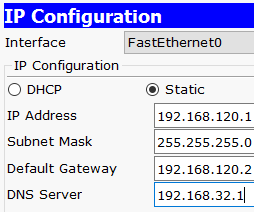
\includegraphics[scale = 0.85]{images/6_2.png}
\end{figure}

\subsection{Настройка сервисов}

Настройка DNS сервиса на узле 192.168.32.1:

\begin{figure}[h!]
	\centering
	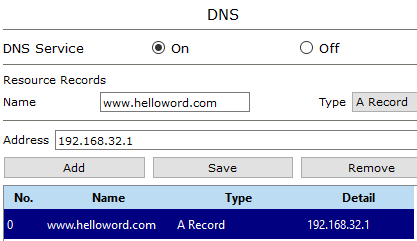
\includegraphics[scale = 1.35]{images/7.png}
	\caption{Настройка DNS сервиса}
\end{figure}

HTTP сервис на узле 192.168.32.1 уже настроен по умолчанию.

\clearpage

Настройка DHCP сервиса на узле 192.168.80.1:

\begin{figure}[h!]
	\centering
	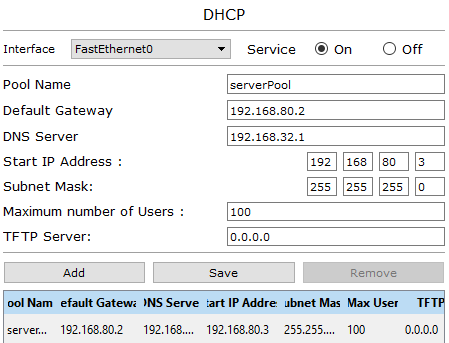
\includegraphics[scale = 1.15]{images/9.png}
	\caption{Настройка DHCP сервиса}
\end{figure}

TFTP сервис на узле 192.168.120.1 уже настроен по умолчанию.

\subsection{Проверка работоспособности}

На узле 192.168.40.32 перейдем по локальному адресу www.helloword.com для проверки работоспособности DNS и HTTP сервисов:

\begin{figure}[h!]
	\centering
	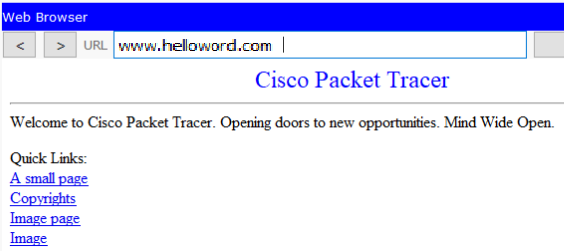
\includegraphics[scale = 1.15]{images/10.png}
	\caption{Тестирование работоспособности DNS и HTTP сервисов}
\end{figure}

\clearpage

На узле 192.168.40.32 (подсеть NET\_1) проверим доступность подсети NET\_4:

\begin{figure}[h!]
	\centering
	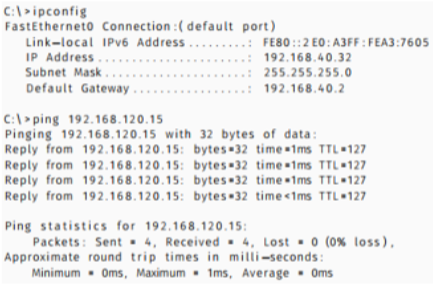
\includegraphics[scale = 0.95]{images/11.png}
	\caption{Настройка DHCP сервиса}
\end{figure}

\section{Вывод}

Cisco Packet Tracer представляет собой удобный инструмент для построения макетов сетей, предоставляя множество инструментов для настройки узлов сети. Большим преимуществом можно считать множество готовых решений, особенно в плане реализации популярных сетевых сервисов.

\end{document}